\documentclass[]{article}
\usepackage{lmodern}
\usepackage{amssymb,amsmath}
\usepackage{ifxetex,ifluatex}
\usepackage{fixltx2e} % provides \textsubscript
\ifnum 0\ifxetex 1\fi\ifluatex 1\fi=0 % if pdftex
  \usepackage[T1]{fontenc}
  \usepackage[utf8]{inputenc}
\else % if luatex or xelatex
  \ifxetex
    \usepackage{mathspec}
  \else
    \usepackage{fontspec}
  \fi
  \defaultfontfeatures{Ligatures=TeX,Scale=MatchLowercase}
\fi
% use upquote if available, for straight quotes in verbatim environments
\IfFileExists{upquote.sty}{\usepackage{upquote}}{}
% use microtype if available
\IfFileExists{microtype.sty}{%
\usepackage{microtype}
\UseMicrotypeSet[protrusion]{basicmath} % disable protrusion for tt fonts
}{}
\usepackage[margin=1in]{geometry}
\usepackage{hyperref}
\hypersetup{unicode=true,
            pdftitle={Supervisor Timesheets},
            pdfborder={0 0 0},
            breaklinks=true}
\urlstyle{same}  % don't use monospace font for urls
\usepackage{graphicx,grffile}
\makeatletter
\def\maxwidth{\ifdim\Gin@nat@width>\linewidth\linewidth\else\Gin@nat@width\fi}
\def\maxheight{\ifdim\Gin@nat@height>\textheight\textheight\else\Gin@nat@height\fi}
\makeatother
% Scale images if necessary, so that they will not overflow the page
% margins by default, and it is still possible to overwrite the defaults
% using explicit options in \includegraphics[width, height, ...]{}
\setkeys{Gin}{width=\maxwidth,height=\maxheight,keepaspectratio}
\IfFileExists{parskip.sty}{%
\usepackage{parskip}
}{% else
\setlength{\parindent}{0pt}
\setlength{\parskip}{6pt plus 2pt minus 1pt}
}
\setlength{\emergencystretch}{3em}  % prevent overfull lines
\providecommand{\tightlist}{%
  \setlength{\itemsep}{0pt}\setlength{\parskip}{0pt}}
\setcounter{secnumdepth}{0}
% Redefines (sub)paragraphs to behave more like sections
\ifx\paragraph\undefined\else
\let\oldparagraph\paragraph
\renewcommand{\paragraph}[1]{\oldparagraph{#1}\mbox{}}
\fi
\ifx\subparagraph\undefined\else
\let\oldsubparagraph\subparagraph
\renewcommand{\subparagraph}[1]{\oldsubparagraph{#1}\mbox{}}
\fi

%%% Use protect on footnotes to avoid problems with footnotes in titles
\let\rmarkdownfootnote\footnote%
\def\footnote{\protect\rmarkdownfootnote}

%%% Change title format to be more compact
\usepackage{titling}

% Create subtitle command for use in maketitle
\newcommand{\subtitle}[1]{
  \posttitle{
    \begin{center}\large#1\end{center}
    }
}

\setlength{\droptitle}{-2em}

  \title{Supervisor Timesheets}
    \pretitle{\vspace{\droptitle}\centering\huge}
  \posttitle{\par}
    \author{}
    \preauthor{}\postauthor{}
    \date{}
    \predate{}\postdate{}
  
\usepackage{booktabs}
\usepackage{longtable}
\usepackage{array}
\usepackage{multirow}
\usepackage[table]{xcolor}
\usepackage{wrapfig}
\usepackage{float}
\usepackage{colortbl}
\usepackage{pdflscape}
\usepackage{tabu}
\usepackage{threeparttable}
\usepackage{threeparttablex}
\usepackage[normalem]{ulem}
\usepackage{makecell}

\begin{document}
\maketitle

The following PDF is an example of the work that can be done with R to
automate the reporting of the \emph{c5 Supervisor} project.

When a member of the Steering committee inputs their task, it updates
the Google spreadsheet. Then, this report works behind the scenes to
access the spreadsheet and find insights that are otherwise hidden. For
example, the following graph shows how many tasks were inputted by
members of the committee:

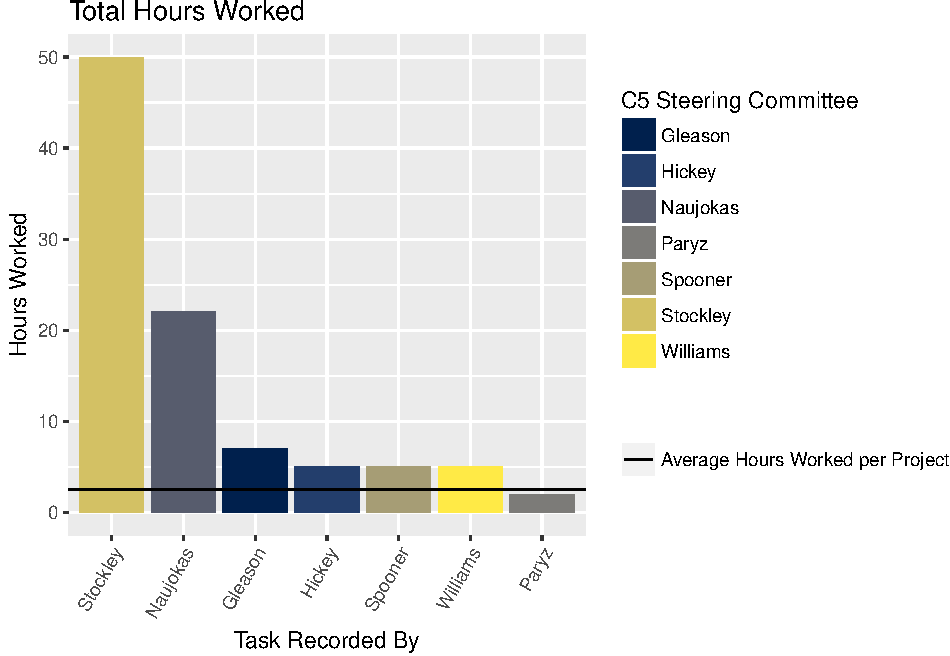
\includegraphics{reports_files/figure-latex/hours_worked-1.pdf}

Automating the report does not just cut down on errors by eliminating
the cut/copy-paste-from-a-spreadsheet-to-a-word-document step. It also
allows for customization. First and foremost, the graph's labels can be
edited, and the color scheme can be set to a color-blind friendly scheme
(see above graph for evidence). Additionally, this report can also fix
DCPO Spooner's name so she is attributed accordingly.

All of the names in the document stem from the email addresses used in
the form. The reason is simple: Most emails are
\texttt{firstname.lastname@cookcountyil.gov}. This allows for a simple
function to split the first and last name. DCPO Spooner, however,
presents a challenge as her email is
\texttt{melissa.parise@cookcountyil.gov}. Fixing this would be time
consuming in the spreadsheet, but given the nature of this report, it is
a trivial task.

In addition to graphs, tables can also be added: \newpage
\rowcolors{2}{gray!6}{white}

\begin{table}

\caption{\label{tab:tasks_count}Person Hours: C5 Project April 2018 - May 2018}
\centering
\begin{tabular}[t]{l|l|r|r}
\hiderowcolors
\hline
first\_name & last\_name & Tasks\_entered & total\_hours\\
\hline
\showrowcolors
Kevin & Hickey & 4 & 5.0\\
\hline
Martin & Gleason & 3 & 7.0\\
\hline
Melissa & Spooner & 1 & 5.0\\
\hline
Nicole & Paryz & 1 & 2.0\\
\hline
Nicole & Williams & 6 & 9.5\\
\hline
Richard & Naujokas & 9 & 26.0\\
\hline
Tamar & Stockley & 19 & 50.0\\
\hline
\end{tabular}
\end{table}

\rowcolors{2}{white}{white} This table summarizes the tasks accomplished
quickly.

\begin{table}[!h]

\caption{\label{tab:person_hours}Total Tasks and Hours}
\centering
\begin{tabular}[t]{r|r}
\hline
Tasks Entered &  Total Hours\\
\hline
43 & 104.5\\
\hline
\end{tabular}
\end{table}

The above table can also be cited within the text. For instance, the
total number of tasks are 43 and the total hours worked on the project
to date is 104.5. This allows for pulling specific insights into the
body of the text, without needing to pull additional information.

Lastly, the tables could be grouped by date. \rowcolors{2}{pink}{white}

\begin{table}[!h]

\caption{\label{tab:table_by_dates}Task per Month}
\centering
\begin{tabular}[t]{l|l|r|r}
\hiderowcolors
\hline
last\_name & Month Completed & Number of Projects & Total Hours Per Month\\
\hline
\showrowcolors
Gleason & May & 3 & 7.0\\
\hline
Hickey & Mar & 1 & 2.0\\
\hline
Hickey & Apr & 2 & 2.0\\
\hline
Hickey & May & 1 & 1.0\\
\hline
Naujokas & Apr & 1 & 14.0\\
\hline
Naujokas & May & 6 & 8.0\\
\hline
Naujokas & Jun & 2 & 4.0\\
\hline
Paryz & Mar & 1 & 2.0\\
\hline
Spooner & Mar & 1 & 5.0\\
\hline
Stockley & Mar & 7 & 13.0\\
\hline
Stockley & Apr & 12 & 37.0\\
\hline
Williams & Mar & 1 & 2.0\\
\hline
Williams & Apr & 1 & 1.0\\
\hline
Williams & May & 3 & 5.0\\
\hline
Williams & Jun & 1 & 1.5\\
\hline
\end{tabular}
\end{table}

\rowcolors{2}{white}{white} This would allow for quick, easy, and
repeateable reporting with a few extra lines of code, all without having
to cut and paste between Excel/Google Sheets and Word. In short, if the
spreadsheet captures the data, then this report can transform it into
the information required by the Steering Committee.


\end{document}
